% Modelo IEEE de conferência. Compila no Overleaf com pdfLaTeX (IEEEtran já vem instalado).
% Seções e regras seguem o enunciado do trabalho final (prof. Michel Pires da Silva, entrega 22/11/2026).
% Só títulos e listas do que escrever. As referências em referencias.bib foram conferidas pelo DOI;
% conferir cada uma no scholar.google.com antes de entregar. Só conta referência citada no texto.
\documentclass[conference]{IEEEtran}
\usepackage[utf8]{inputenc}
\usepackage[T1]{fontenc}
\usepackage[brazil]{babel}
\usepackage{amsmath}
\usepackage{graphicx}
\usepackage{booktabs}
\usepackage{url}
\usepackage{tikz}
\usetikzlibrary{positioning, arrows.meta}

% lista do que escrever em cada seção. apagar antes de entregar
\newcommand{\escrever}[1]{\noindent\textbf{A escrever:}\begin{itemize}\setlength\itemsep{0pt}#1\end{itemize}}

\begin{document}

\title{Recomendação de Roupas com KD-tree e Grafos}

% alunos por contribuição decrescente (igual: ordem alfabética); o professor é sempre o último
\author{
\IEEEauthorblockN{Maria Eduarda Alves Barbosa}
\IEEEauthorblockA{Engenharia de Computação\\CEFET-MG, Campus Divinópolis\\Divinópolis, MG, Brasil}
\and
\IEEEauthorblockN{Igor Moreira Lopes}
\IEEEauthorblockA{Engenharia de Computação\\CEFET-MG, Campus Divinópolis\\Divinópolis, MG, Brasil}
\and
\IEEEauthorblockN{Michel Pires da Silva}
\IEEEauthorblockA{CEFET-MG\\Divinópolis, MG, Brasil}
}

\maketitle

\begin{abstract}
\escrever{
\item um parágrafo, no máximo 250 palavras, respondendo nesta ordem:
\item qual o problema: completar um look com uma peça de outra categoria;
\item há soluções? quais: redes neurais de compatibilidade (Bi-LSTM, embeddings por tipo) e filtragem por item;
\item como foi modelado: KD-tree, grafo peça--look com BFS, Union-Find, Kruskal, Tarjan, sobre a FashionVerse-MME (102.370 peças, 31.333 looks);
\item principal resultado, com números da Tabela~\ref{tab:final}, e a limitação da peça nova (Tabela~\ref{tab:conhecida_nova}).
}
\end{abstract}

\begin{IEEEkeywords}
\escrever{\item 4 a 6 palavras-chave.}
\end{IEEEkeywords}

\section{Introdução}
\escrever{
\item funil: começar pelo cenário amplo (comércio de moda, sistemas de recomendação) e afunilar até completar um look;
\item por que o problema importa no mundo real (exemplo concreto de uso);
\item motivação da equipe para o tema;
\item objetivos principais, declarados sem ambiguidade;
\item por que estruturas clássicas (leve e explicável);
\item contribuições: versões A a F, avaliação justa, base tratada no Zenodo~\cite{zenodo}, código aberto~\cite{repositorio};
\item parágrafo-roteiro: o que vem em cada seção e o que se espera alcançar.
}

\section{Referencial Teórico (Estado da Arte)}
\escrever{
\item o que a literatura diz sobre o problema: compatibilidade de roupas com Bi-LSTM e FITB~\cite{han2017}, embeddings por tipo de peça~\cite{vasileva2018}, recomendação por imagem de estilos e substitutos~\cite{mcauley2015};
\item recomendação top-$N$ baseada em itens e a métrica Hit@k~\cite{deshpande2004};
\item KD-tree: construção, busca kNN e custo esperado~\cite{bentley1975,friedman1977};
\item grafo peça--look e BFS de 2 passos;
\item Union-Find com união por tamanho e compressão de caminho~\cite{galler1964,tarjan1975};
\item árvore geradora mínima: Kruskal e Prim~\cite{kruskal1956,prim1957}; agrupamento por AGM e efeito corrente~\cite{zahn1971,gower1969};
\item grafo de condensação (grupos como supervértices) e grau do vértice (popularidade);
\item Tarjan: pontes e vértices de articulação~\cite{tarjan1972,hopcroft1973};
\item NP-dificuldade de montar o look inteiro, por redução da clique~\cite{karp1972} (\texttt{docs/VERSAO\_F.md}, seção 4).
}

\section{Metodologia}
\escrever{
\item origem e natureza dos dados: FashionVerse-MME~\cite{fashionverse}, licença, o que cada registro tem;
\item pré-processamento e junção de registros repetidos;
\item modelagem: o que é vértice e o que é aresta em cada grafo (peça--look, kNN mútuo, grupos), e o que é nó na KD-tree;
\item atributos do texto e acerto contra a referência rotulada pela imagem;
\item lógica do algoritmo passo a passo, seguindo o fluxograma (Fig.~\ref{fig:fluxo});
\item versões A, B, C, D e F (a final) e a fórmula da nota;
\item pontos por atributo: $\log((n+1)/(\text{esperado}+1))$;
\item por que as peças gêmeas não entraram (24 de 50 pares).
}

\begin{figure}[t]
\centering
\resizebox{\columnwidth}{!}{% fluxograma da metodologia. cada caixa aponta o script ou comando do repositorio
\begin{tikzpicture}[
  node distance=4mm,
  caixa/.style={draw, rounded corners=2pt, align=center, font=\scriptsize, minimum width=7.6cm, inner sep=3pt},
  dado/.style={draw, align=center, font=\scriptsize, minimum width=7.6cm, inner sep=3pt, fill=black!6},
  seta/.style={-{Latex[length=2mm]}, semithick}]
\node[dado] (base) {FashionVerse-MME: 126.928 registros em 31.333 looks (JSON)};
\node[caixa, below=of base] (pre) {Pré-processamento: junta registros repetidos (102.370 peças),\\cor Lab, divisão dos looks em treino, validação e teste};
\node[caixa, below=of pre] (atr) {Atributos do texto (estilo, ocasião, formalidade, estampa)\\e 12 grupos de cor com k-means};
\node[caixa, below=of atr] (est) {Estruturas: KD-tree, grafo peça--look (BFS de 2 passos),\\Union-Find e Kruskal (grupos), tabelas de pontos};
\node[caixa, below=of est] (ver) {Versões A, B, C, D e F: nota para todas as peças\\da categoria da peça escondida};
\node[caixa, below=of ver] (val) {Validação: escolhe pesos e parâmetros\\(metade A escolhe, metade B confirma)};
\node[caixa, below=of val] (tes) {Teste único: Hit@1, Hit@5, Hit@10 e FITB,\\10 ordens de desempate e bootstrap};
\node[dado, below=of tes] (sai) {Tabelas, gráficos de tempo, Gephi e articulações (Tarjan)};
\foreach \a/\b in {base/pre, pre/atr, atr/est, est/ver, ver/val, val/tes, tes/sai} \draw[seta] (\a) -- (\b);
\end{tikzpicture}
}
\caption{Fluxograma da proposta, da entrada dos dados até os resultados.}
\label{fig:fluxo}
\end{figure}

\subsection{Configuração experimental}
\escrever{
\item ambiente: Ubuntu 22.04.5, g++ 11.4, 8 núcleos, carga da máquina; o enunciado exige Ubuntu 24.04: testar lá antes de escrever;
\item como rodar: \texttt{make demo}, instruções no repositório~\cite{repositorio};
\item divisão treino, validação e teste e sementes;
\item avaliação justa: categoria inteira, 10 ordens de desempate, Hit@k e FITB;
\item escolha só na validação, metades A e B, teste usado uma vez por configuração;
\item bootstrap com 1.000 sorteios~\cite{efron1979};
\item testes de tempo: $n = 10^3$, $10^4$ e $10^5$, 5 repetições.
}

\section{Resultados e Discussão}
\escrever{
\item Tabela~\ref{tab:final}: comparação de todas as versões;
\item Tabela~\ref{tab:diferencas}: o que é diferença real e o que pode ser sorte;
\item Tabela~\ref{tab:conhecida_nova}: peça conhecida contra peça nova;
\item Tabela~\ref{tab:tempos} e Fig.~\ref{fig:tempos}: teoria contra prática; como cada estrutura se comportou quando a entrada cresceu;
\item qual foi o gargalo e por quê;
\item Fig.~\ref{fig:grupos}: grupos e articulações, desenhados no Gephi~\cite{bastian2009} com ForceAtlas2~\cite{jacomy2014};
\item discutir criticamente: o que os números significam, não só mostrar;
\item experimento registrado, fora da versão final: F2 pelo FITB e as tentativas para a peça nova (\texttt{docs/VERSAO\_F.md}, seção 8).
}

\begin{table}[t]
\centering
\caption{Teste com 5.842 looks: média de 10 ordens de desempate (tabela\_final.md).}
\label{tab:final}
\footnotesize
\begin{tabular}{lrrrr}
\toprule
Versão & Hit@1 & Hit@5 & Hit@10 & FITB \\
\midrule
Aleatória (esperado) & 0,018\% & 0,091\% & 0,182\% & 25,00\% \\
Popularidade & 0,142\% & 0,568\% & 0,895\% & 31,40\% \\
A & 0,051\% & 0,188\% & 0,514\% & 34,29\% \\
B & 0,373\% & 0,647\% & 0,772\% & 25,35\% \\
C & 0,336\% & 0,633\% & 0,751\% & 25,37\% \\
D & 0,329\% & 0,531\% & 0,659\% & 28,14\% \\
D nova & 0,312\% & 0,575\% & 0,688\% & 27,26\% \\
C + popularidade & 0,313\% & 0,746\% & 1,058\% & 31,63\% \\
F & 0,313\% & 0,716\% & 1,056\% & 32,04\% \\
\bottomrule
\end{tabular}
\end{table}

\begin{table*}[t]
\centering
\caption{Diferenças no teste, em pontos percentuais, com intervalo de 95\% (bootstrap, 1.000 sorteios).}
\label{tab:diferencas}
\footnotesize
\begin{tabular}{lrrrr}
\toprule
Comparação & Métrica & Diferença & Intervalo & Conclusão \\
\midrule
F x Popularidade & Hit@10 & 0,161 & $-$0,068 a 0,383 & pode ser sorte \\
F x Popularidade & FITB & 0,63 & 0,14 a 1,11 & real \\
F x C & Hit@10 & 0,305 & 0,113 a 0,510 & real \\
F x C & FITB & 6,67 & 5,90 a 7,43 & real \\
F x C + popularidade & Hit@10 & $-$0,002 & $-$0,015 a 0,010 & pode ser sorte \\
F x C + popularidade & FITB & 0,41 & $-$0,05 a 0,86 & pode ser sorte \\
\bottomrule
\end{tabular}
\end{table*}

\begin{table*}[t]
\centering
\caption{Peça escondida conhecida (1.600 consultas) e nova (4.242), no teste. x = vezes o aleatório.}
\label{tab:conhecida_nova}
\footnotesize
\begin{tabular}{lrrrrrr}
\toprule
Versão & Hit@10 conh. & x & FITB conh. & Hit@10 nova & x & FITB nova \\
\midrule
Aleatória (esperado) & 0,167\% & 1,0 & 25,00\% & 0,187\% & 1,0 & 25,00\% \\
Popularidade & 3,269\% & 19,5 & 47,99\% & 0,000\% & 0,0 & 25,14\% \\
A & 0,438\% & 2,6 & 32,13\% & 0,542\% & 2,9 & 35,10\% \\
B & 2,331\% & 13,9 & 25,89\% & 0,184\% & 1,0 & 25,14\% \\
C & 2,394\% & 14,3 & 25,97\% & 0,132\% & 0,7 & 25,14\% \\
D & 1,781\% & 10,6 & 30,39\% & 0,236\% & 1,3 & 27,28\% \\
D nova & 1,856\% & 11,1 & 29,14\% & 0,248\% & 1,3 & 26,56\% \\
C + popularidade & 3,863\% & 23,1 & 48,83\% & 0,000\% & 0,0 & 25,14\% \\
F & 3,856\% & 23,0 & 49,04\% & 0,000\% & 0,0 & 25,62\% \\
F2 (FITB) & 3,825\% & 22,8 & 53,54\% & 0,000\% & 0,0 & 37,15\% \\
\bottomrule
\end{tabular}
\end{table*}

\begin{table}[t]
\centering
\caption{Tempos em ms, média de 5 repetições (tempos\_f.md).}
\label{tab:tempos}
\footnotesize
\begin{tabular}{lrrr}
\toprule
Medida & $n=10^3$ & $n=10^4$ & $n=10^5$ \\
\midrule
Construir a KD-tree & 0,2315 & 2,876 & 48,98 \\
kNN na KD-tree (consulta) & 0,007219 & 0,01299 & 0,09484 \\
kNN força bruta (consulta) & 0,0117 & 0,07875 & 1,343 \\
Union-Find sem técnicas & 3,458 & 297,6 & 29.204 \\
Union-Find com técnicas & 0,009074 & 0,07919 & 0,7813 \\
Kruskal: ordenar & 0,3545 & 4,328 & 51,73 \\
Kruskal: uniões & 0,04993 & 0,4981 & 6,523 \\
Prim com heap & 0,5577 & 8,527 & 105,7 \\
BFS 2 passos (consulta) & 0,000017 & 0,000067 & 0,000367 \\
\bottomrule
\end{tabular}
\end{table}


\begin{figure*}[t]
\centering
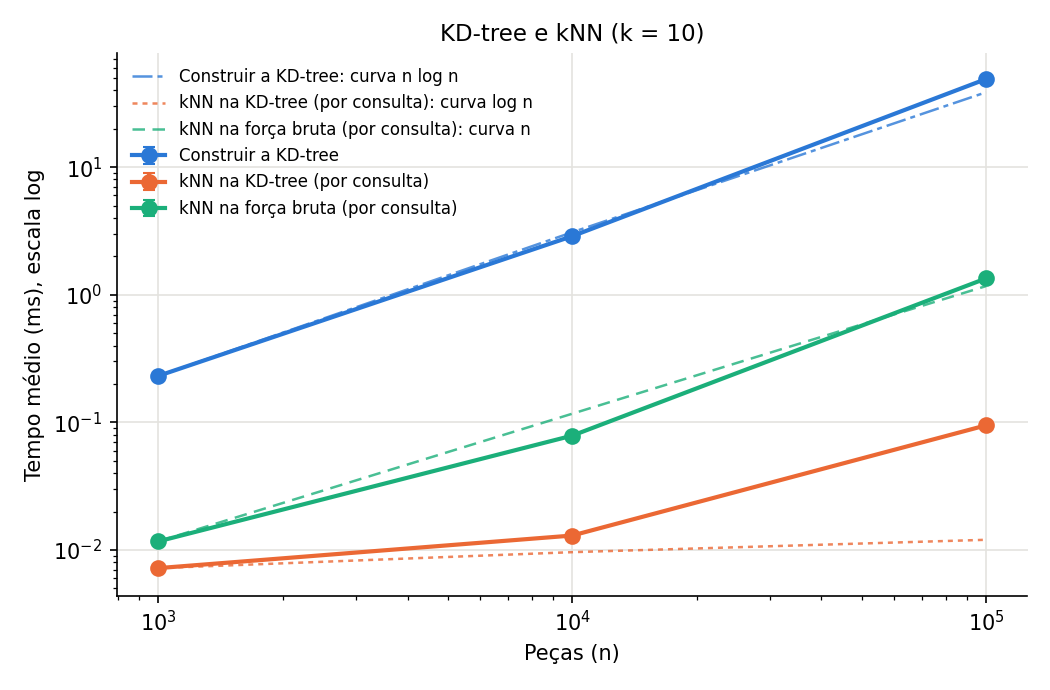
\includegraphics[width=0.24\textwidth]{figuras/kdtree.png}\hfill
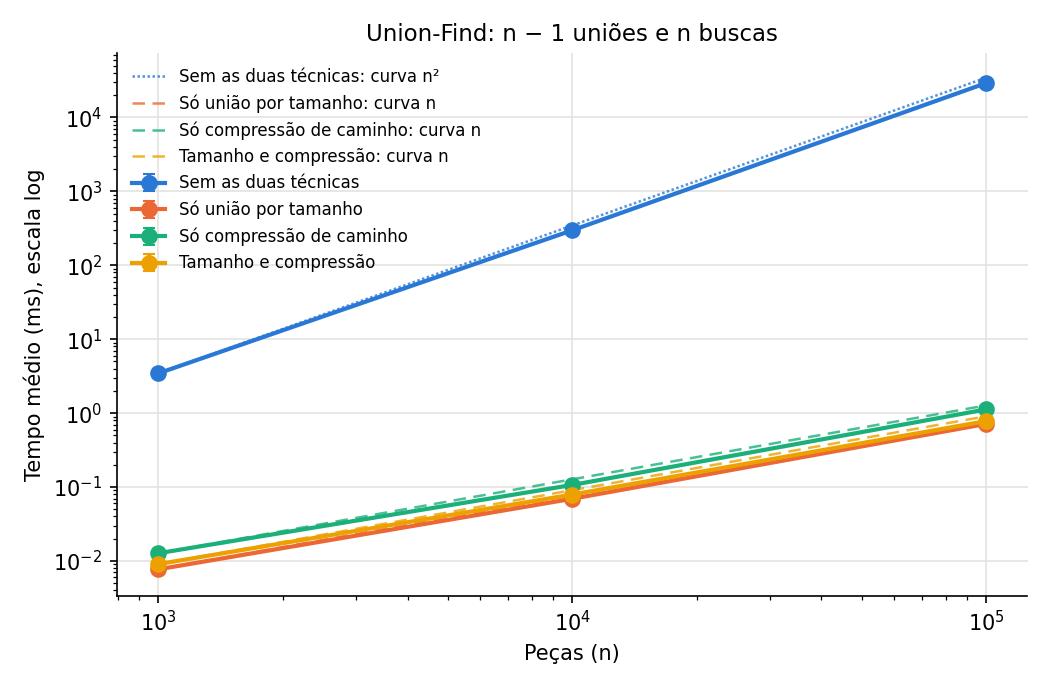
\includegraphics[width=0.24\textwidth]{figuras/union_find.png}\hfill
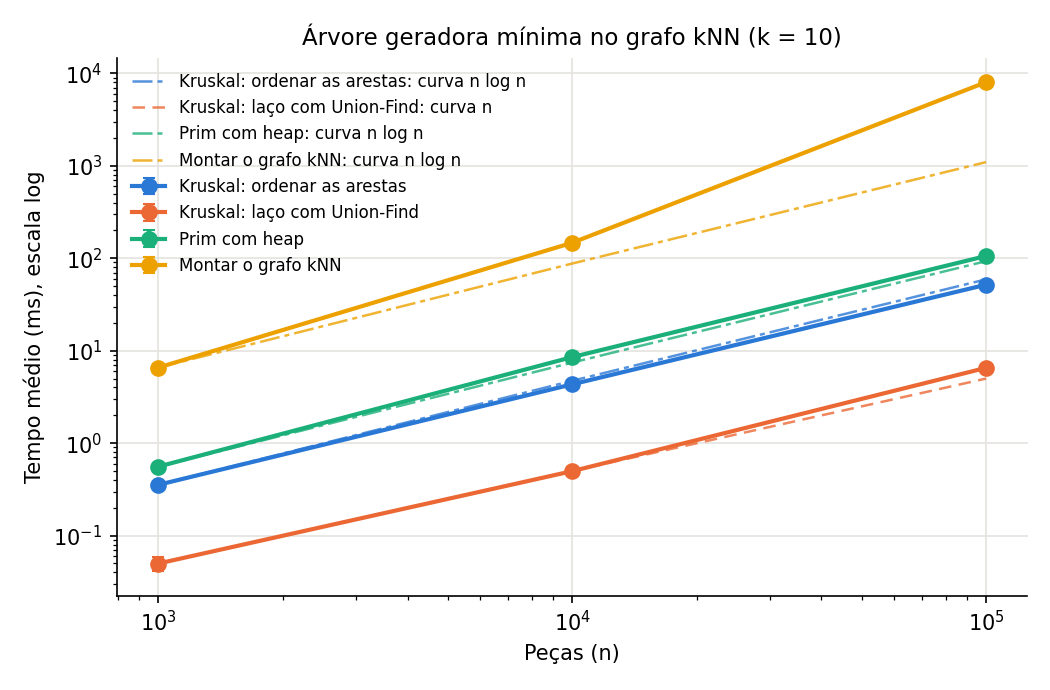
\includegraphics[width=0.24\textwidth]{figuras/agm.png}\hfill
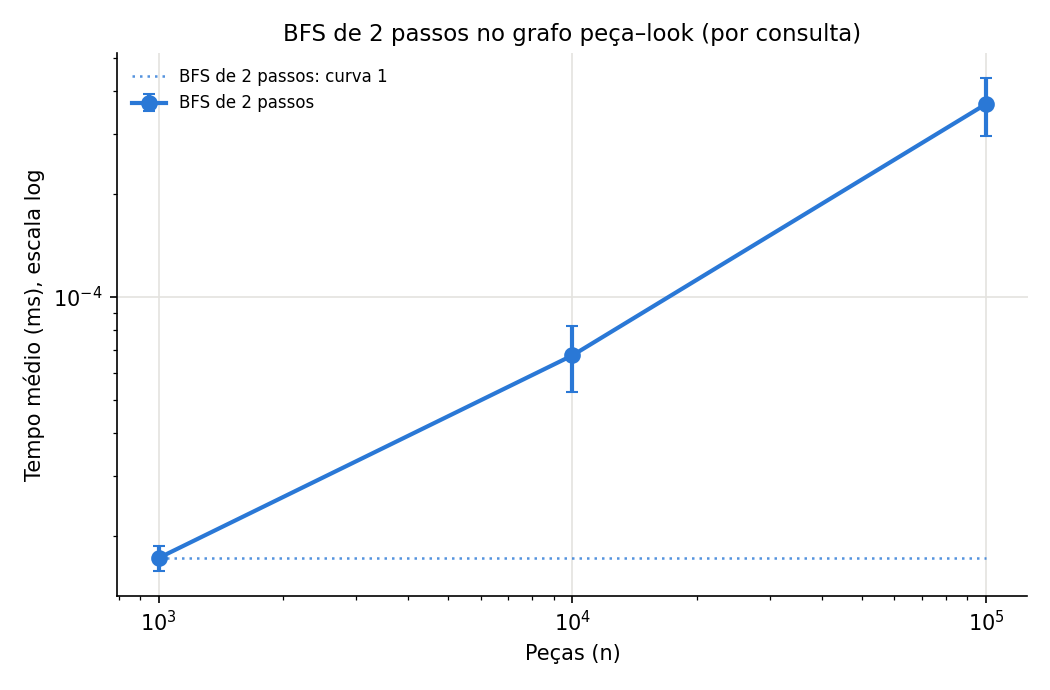
\includegraphics[width=0.24\textwidth]{figuras/bfs.png}
\caption{Tempo por tamanho da base, em escala log-log, com a curva teórica tracejada.}
\label{fig:tempos}
\end{figure*}

\begin{figure}[t]
\centering
% trocar pela imagem do Gephi (resultados/gephi_articulacoes/q2_*), ver LEIA-ME.md
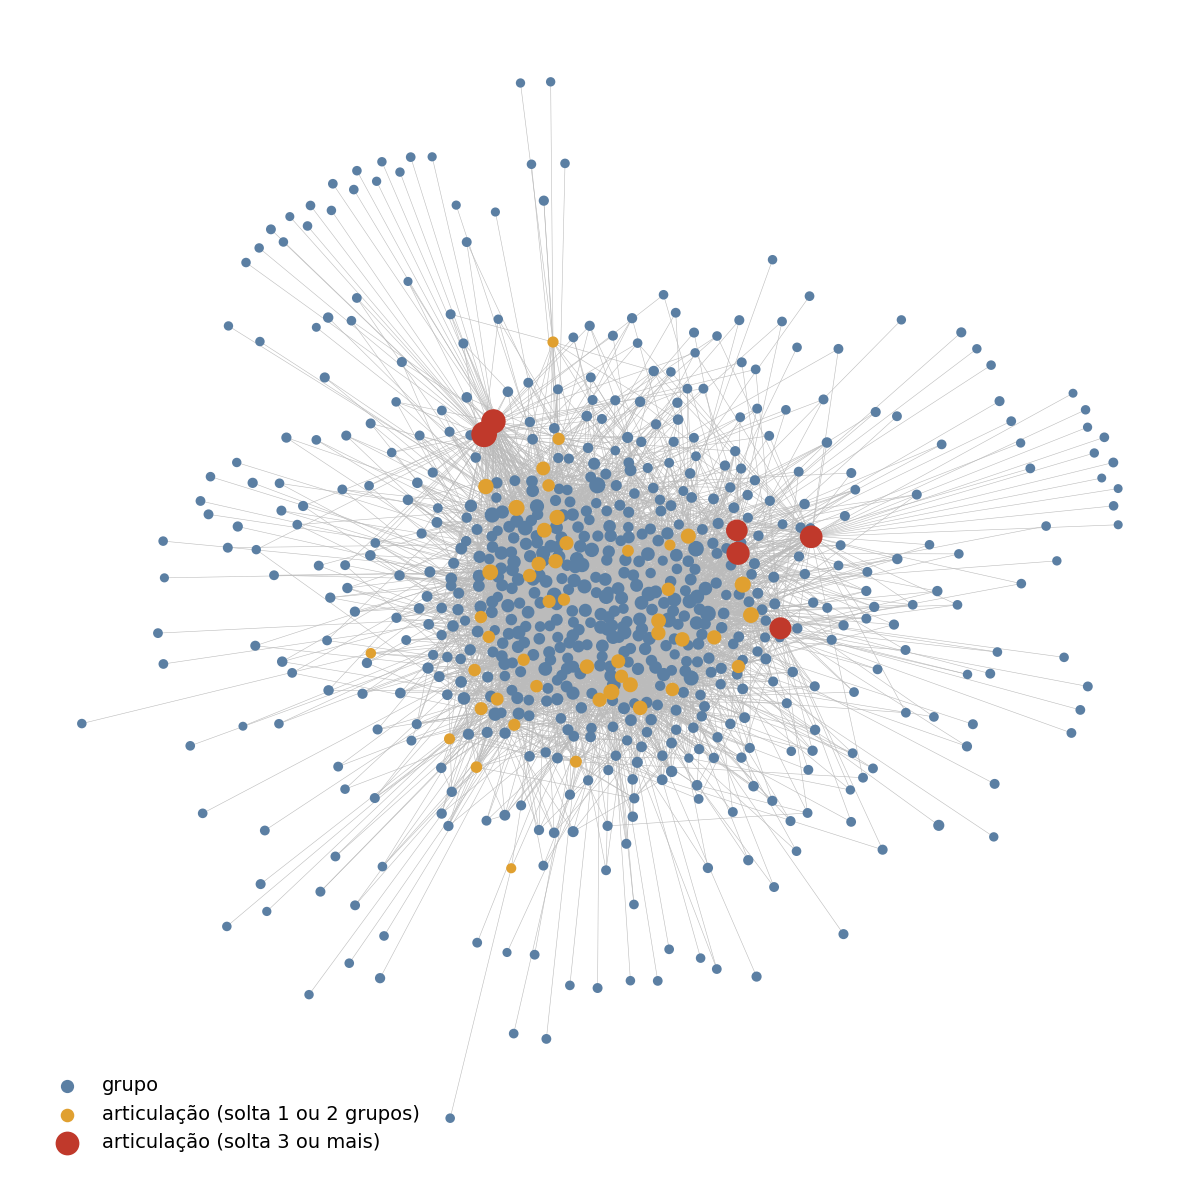
\includegraphics[width=\columnwidth]{figuras/grupos_articulacoes.png}
\caption{Grafo entre grupos com as articulações em destaque.}
\label{fig:grupos}
\end{figure}

\section{Conclusão e Próximas Etapas}
\escrever{
\item contribuições da equipe;
\item desafios e limitações: 72,6\% de peças novas, atributos do texto, efeito corrente;
\item sugestões de melhoria para pesquisas futuras.
}

\bibliographystyle{IEEEtran}
\bibliography{referencias}

\end{document}
